\chapter{Evaluation}
\label{chap:evaluation}
\section{Fuzzing and Results}
Fuzz test is an automated software testing approach feeding inputs to target programs to expose vulnerabilities and fix them in advance. Compared to other vulnerability discovery techniques, the fuzzing test has high accuracy and good scalability.  
Our fuzzing test is based on known data structures and measuring the code coverage, so it is a generation-based and coverage-based fuzzer.\cite{li_zhao_zhang_2018}

Figure \ref{fig:fuzzing} shows the process of fuzzing tests which consists of four main parts, testcase generation, program implementation, program monitoring and violation analysis. So the quality of test cases significantly impacts the testing effects. The inputs should satisfy the properties of data structures as much as possible and, on the other hand, should be wide enough to reveal problems embedded in the software. \cite{li_zhao_zhang_2018}
\begin{figure}[ht]
    \centering
    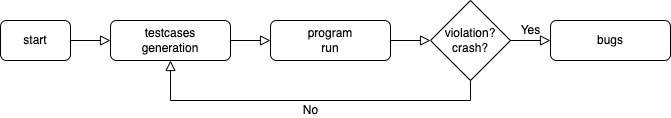
\includegraphics[scale=0.4]{Bilder/fuzz.png}
    \caption{process of fuzzing test}
    \label{fig:fuzzing}
\end{figure}

As the implementation depicted in the section \ref {sec:generator}, our random input generator could satisfy all the testing properties we proposed before and are forced to generate diagrams with \verb|Joint| and at least two levels with great possibility. 
It could generate many and different diagram expressions that even we might have never tried by hand and very rare. 

We take some random data as inputs to our exiting drawing tool. 
Here are some results. The generated component types and transitions in a diagram expression achieve high randomness.

 
\begin{figure}[htbp]
\centering
\begin{minipage}[t]{0.4\textwidth}
\centering
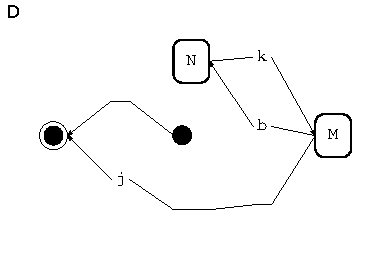
\includegraphics[width=5.5cm]{Bilder/sample3.pdf}
\caption{sample 1}
\end{minipage}
\begin{minipage}[t]{0.4\textwidth}
\centering
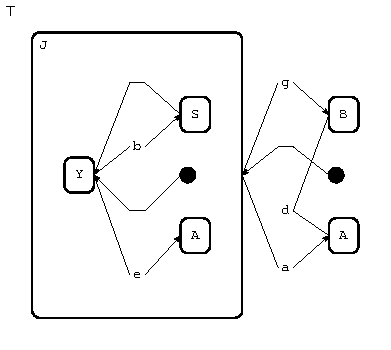
\includegraphics[width=5.5cm]{Bilder/sample1.pdf}
\caption{sample 2}
\end{minipage}
\end{figure}

\begin{figure}[htbp]
\centering
\begin{minipage}[t]{0.48\textwidth}
\centering
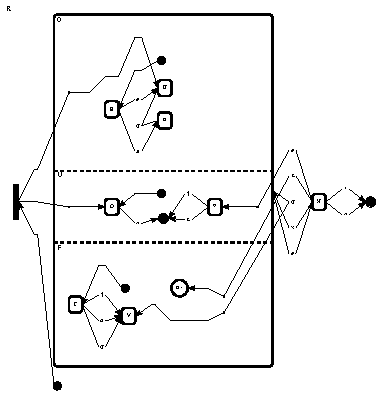
\includegraphics[width=6cm]{Bilder/sample4.pdf}
\caption{sample 3}
\end{minipage}
\begin{minipage}[t]{0.48\textwidth}
\centering
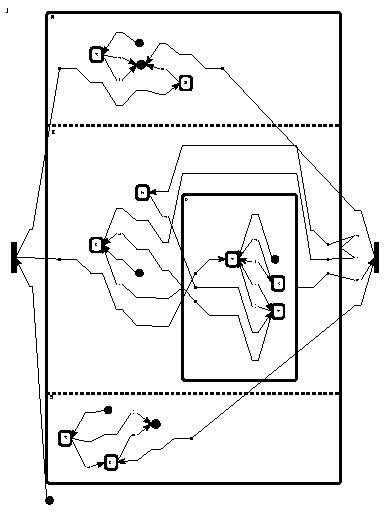
\includegraphics[width=6cm]{Bilder/sample2.pdf}
\caption{sample 4}
\end{minipage}
\end{figure}

After several experimental executions, we found our drawing tool crashed in certain situations and will show two types of errors :

\begin{verbatim}
 sampling.exe: Maybe.fromJust: Nothing
\end{verbatim}
\begin{verbatim}
 sampling: No match in record selector lengthXY
\end{verbatim}

Those errors may be fixed in later work. Here we simply ignore those diagrams that the tool are unable to draw.
The fuzzing test eventually helps us improve the program since our random generator will produce many corner cases that may cause the program to fail.


\section{Coverage Analysis}

 We use the HPC toolkit \cite{gill_runciman_2007} to measure the degree of thoroughness of our test suite.
Figure \ref{fig:coverage1} and \ref{fig:coverage2} gives the code coverage of each module. 

From the code coverage measured by HPC, the average coverage of the top-level definitions is 91$\%$. It is an ideal result since it is reasonable that some codes would not be executed\cite{gill_runciman_2007}.
We have achieved very high coverage on checkers.
However, the coverage on the arrow drawing is deficient.
This could be our future focus.

\begin{figure}[ht]
    \centering
    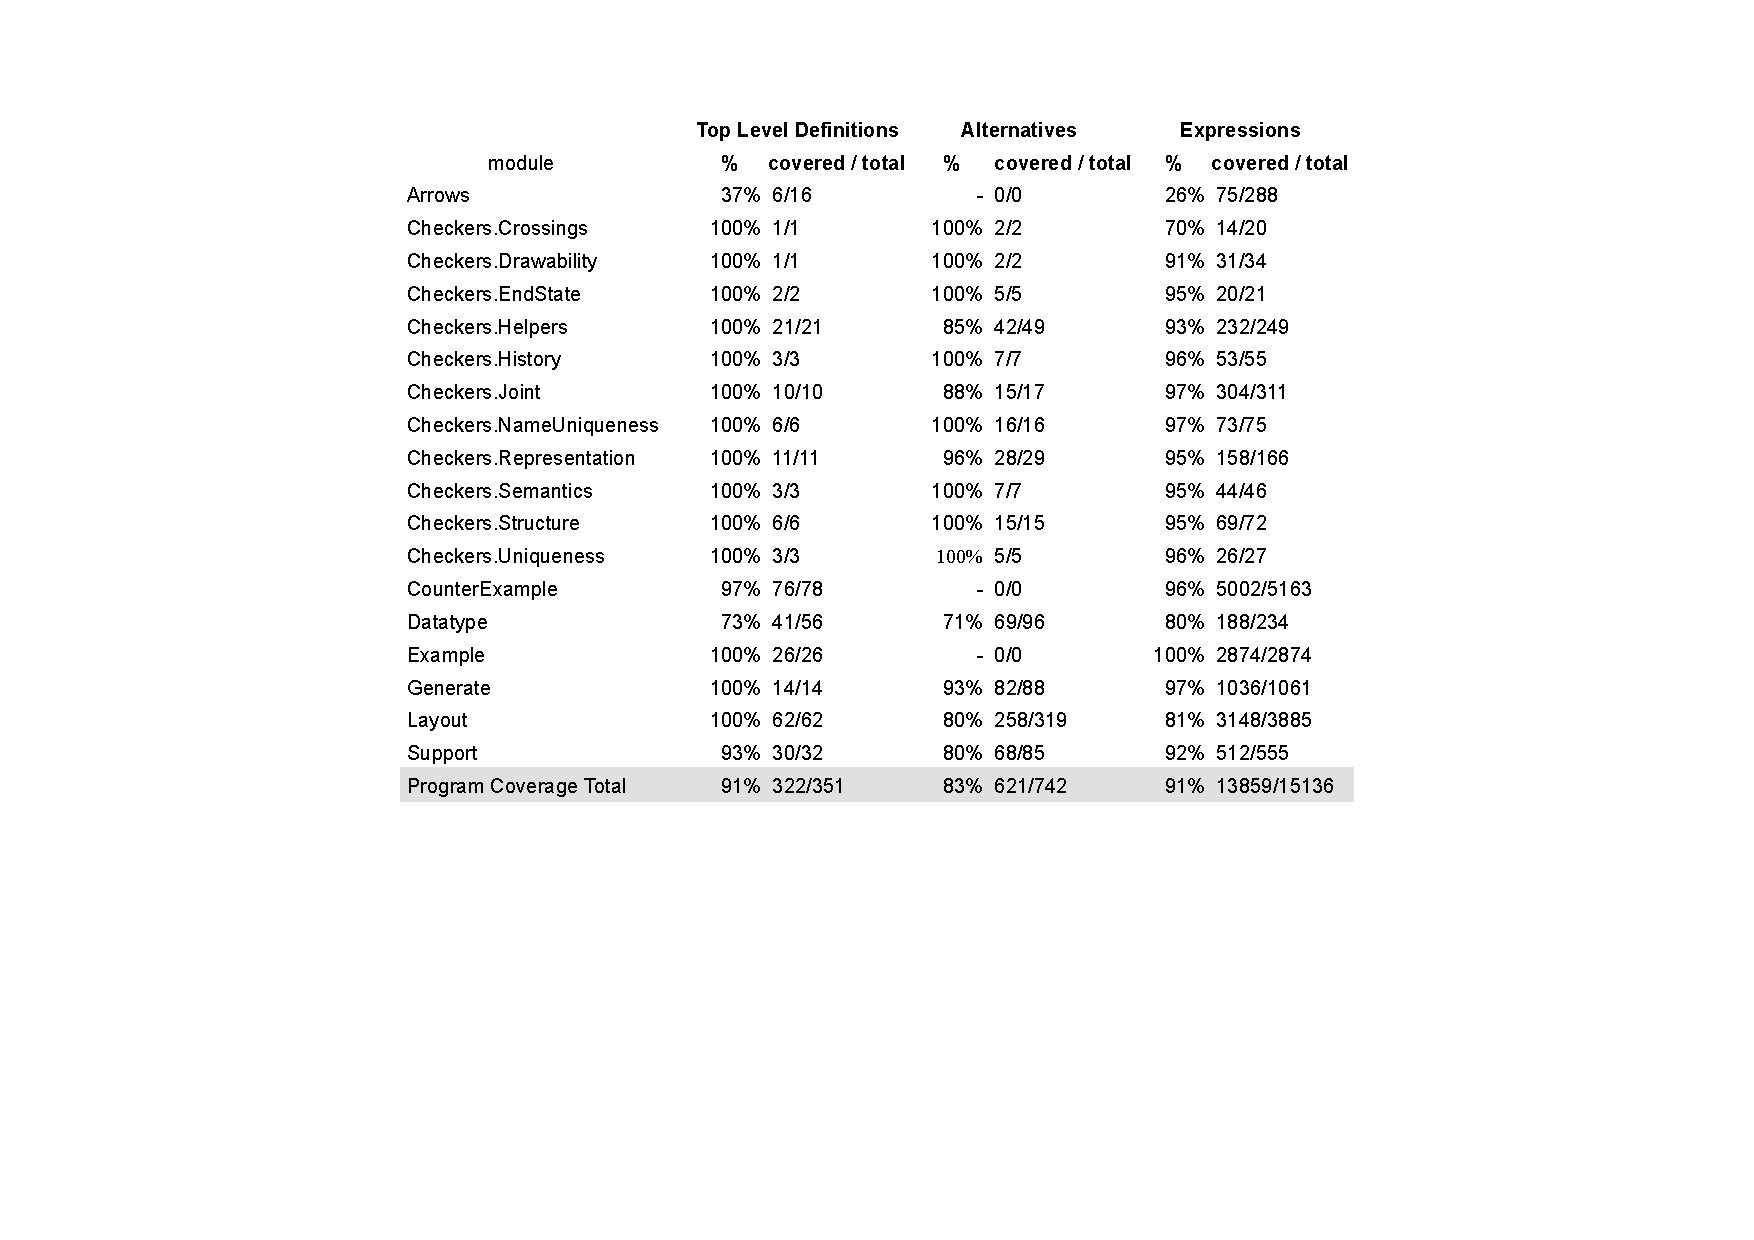
\includegraphics[scale=0.65]{Bilder/coverage1.pdf}
    \caption{coverage output from hpc-markup}
    \label{fig:coverage1}
\end{figure}
\begin{figure}[ht]
    \centering
    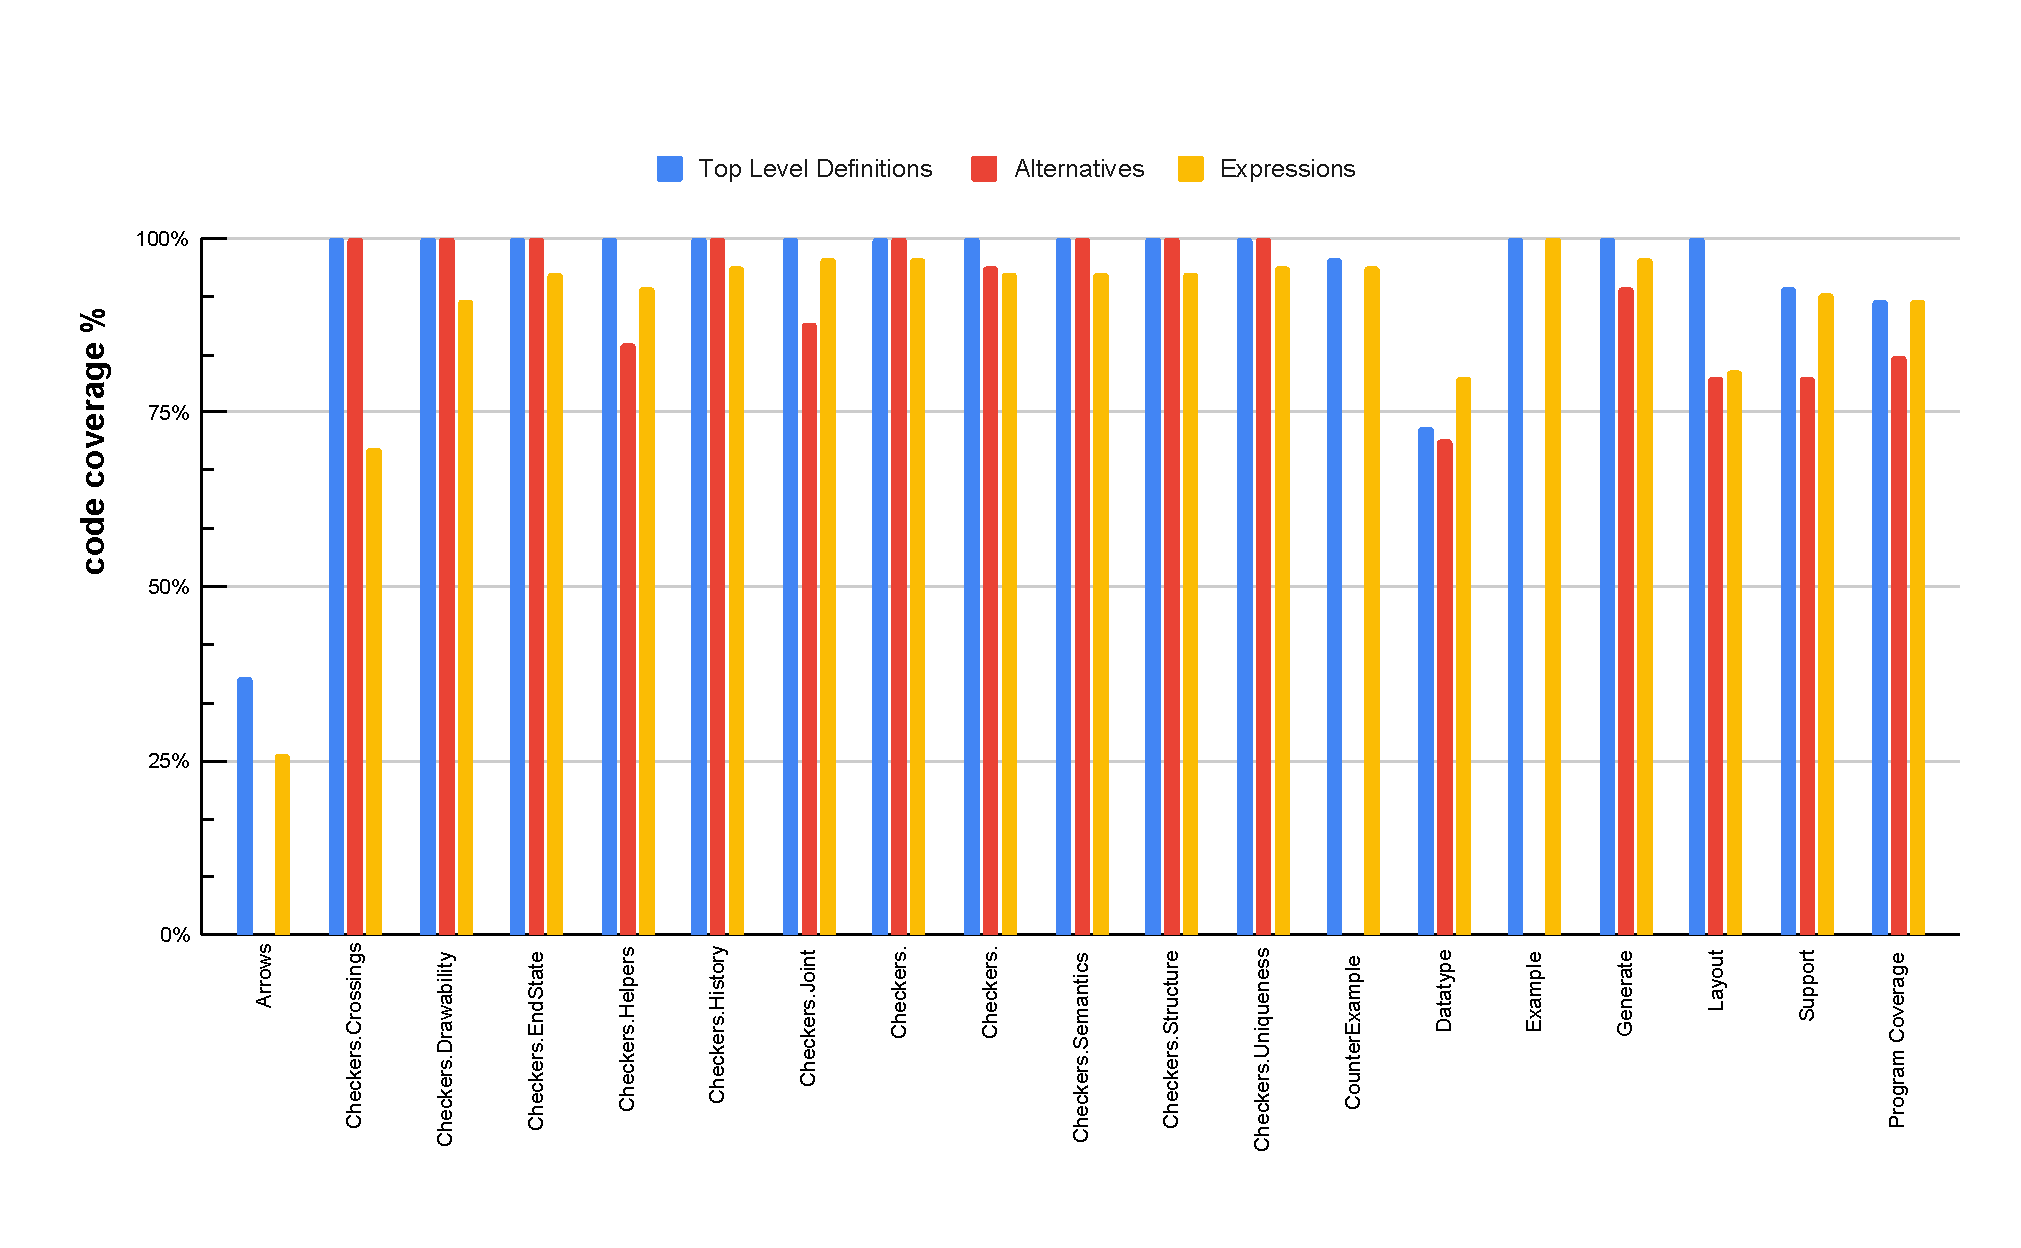
\includegraphics[scale=0.4]{Bilder/coverage2.pdf}
    \caption{coverage}
    \label{fig:coverage2}
\end{figure}
\newpage
\section{Errors Found}
Except for the errors found by fuzzing tests, we encountered another drawing problem by investigating the random generator: discontinuous lines under certain circumstances.At the layer of \verb|StateDiagram C| inside a combine diagram \verb|Connection [2] [4,2,4] "f"| is drawn with a discontinuous line. We might investigate it further in the future.
\begin{figure}[ht]
    \centering
    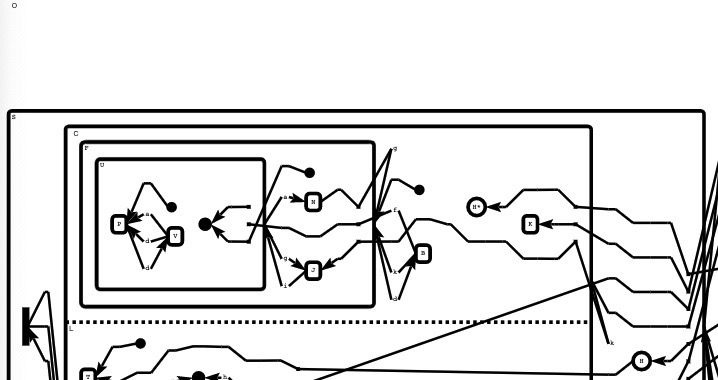
\includegraphics[scale=0.5]{Bilder/error.jpg}
    \caption{discontinuous lines}
    \label{fig:error}
\end{figure}


